\subsection{Quantum Chromodynamics}
The Standard Model of particle physics represents the most complete description of fundamental interactions to date, surviving over 70 years of theoretical and experimental scrutiny.
The Standard Model, shown in Figure~\ref{fig:standard_model_particles}, combines Quantum Field Theories of the electroweak forces and the strong interaction into a unified framework.
Each interaction has its own force carrier, with the strong, electromagnetic, and weak forces being mediated by the gluon, photon, and W$^{\pm}$ and Z bosons, respectively.

\begin{figure}
    \centering
    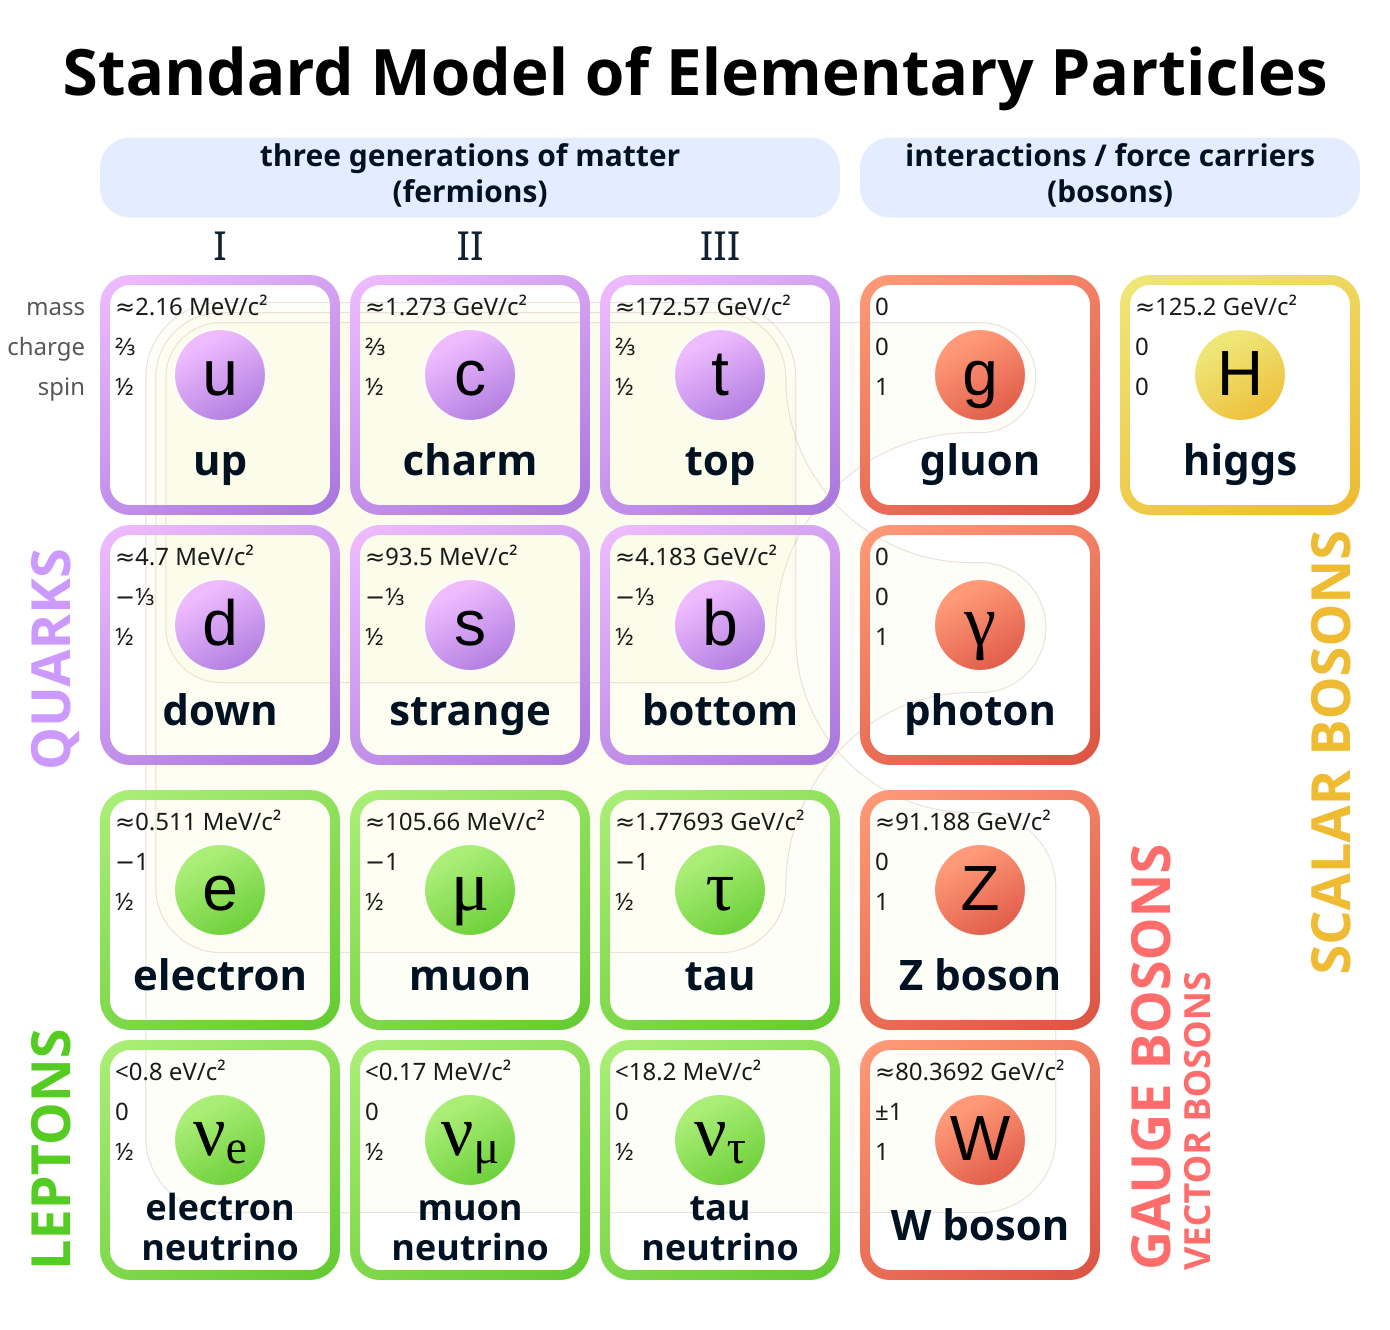
\includegraphics[
        width=0.85\textwidth,
        alt={Diagram of the Standard Model showing three generations of quarks
        and leptons, along with gauge bosons and the Higgs boson.}
    ]{chapters/background/sections/quantum_chromodynamics/figures/standard_model_of_elementary_particles.pdf}
    \caption{The elementary particles and force carriers of the Standard Model.
    Adapted from Ref.~\cite{WikimediaCommonsStandardModel}.}
    \label{fig:standard_model_particles}
\end{figure}

\subsubsection{QCD}
Placeholder text for this section.

\subsubsection{Parton Distribution Functions}
Placeholder text for this section.
